\section{Kompilator}

Kompilacja polega na przetworzeniu kodu źródłowego programu, danego w postaci tekstowej, na wykonywalny plik binarny, który procesor będzie ,,rozumiał'' i potrafił wykonać. Działanie kompilatora składa się z kilku faz, z których każda w jakiś sposób transformuje swoje wejście. Zostały one schematycznie przedstawione na rysunku \ref{fig:CompilerOverview}

\begin{figure}
  \begin{center}
    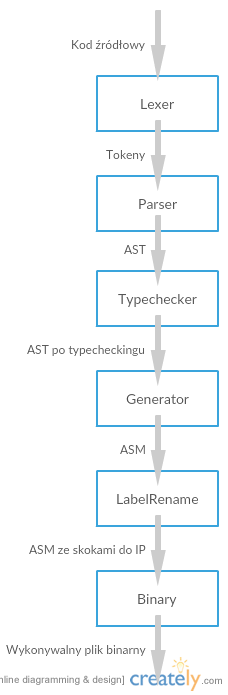
\includegraphics[scale=0.75]{images/CompilerOverview.png}
    \caption{Schemat działania kompilatora. Każda z faz przedstawionych na rysunku jest osobnym modułem, opisanym poniżej.}
    \label{fig:CompilerOverview}
  \end{center}
\end{figure}

\subsection{Moduły w języku Haskell}
Kompilator został stworzony w języku Haskell[1], zatem zanim przejdziemy do opisu poszczególnych modułów, przedstawimy podejście do grupowania kodu w moduły w języku Haskell.

Grupowanie kodu w moduły jest w języku Haskell szczególnie ważne, a klarowna i uporządkowania struktura modułów świadczy o dobrym stylu programowania[2]. Wspominamy o szczególnej ważności, jako że w Haskellu nie ma obiektowości, a nazwy pól w rekordach są globalne dla całego modułu. Przykładowo, nie możemy w jednym pliku stworzyć rekordów typu A i B, posiadających pola o tej samej nazwie (spowoduje to błąd kompilacji). Dobrą praktyką jest zatem nieumieszczanie w jednym module zbyt dużej ilości typów danych, a przy importowaniu modułów kwalifikowanie ich nazw (w przeciwieństwie do wrzucania wszystkich nazw do jednej przestrzeni nazw). Podejście takie jest szczególnie korzystne, gdy kod tworzy więcej osób, które muszą ze sobą współpracować.

Haskell wymusza na nas umieszczanie każdego modułu w osobnym pliku, a na pełną nazwę modułu (podobnie jak np. w języku Java) składa się cała ścieżka (od głównego folderu ze źródłami projektu) oraz nazwa pliku. Przykładowo, jeśli chcemy stworzyć moduł \texttt{A.B.C}, musimy w folderze \texttt{src} naszego projektu umieścić plik \texttt{A/B/C.hs}. Dodatkowo, mamy możliwość importowania modułów na różne sposoby. Rozważmy sytuację, w której chcemy użyć funkcji \texttt{foo} z modułu \texttt{A}, zawierającego również funkcję \texttt{bar}:
\begin{itemize}
  \item \texttt{import A} -- zaimportujemy wszystkie symbole z modułu A do bieżącej przestrzeni nazw (czyli będziemy mogli napisać zarówno: \texttt{foo}, jak \texttt{bar}
  \item \texttt{import A hiding (bar)} -- zaimportujemy cały moduł A, z wyjątkiem funkcji bar
  \item \texttt{import qualified A} -- zaimportujemy cały moduł A, ale w sposób kwalifikowany, tj. będziemy pisać: \texttt{A.foo} i \texttt{A.bar}
  \item \texttt{import A (foo)} -- zaimportujemy jedynie funkcję foo
\end{itemize}

Dobrą praktyką jest stosowanie wyłącznie importów w dwóch ostatnich stylach --- poprawia to czytelność kodu i ułatwia jego współdzielenie. Wyjątkiem są sytuacje, w których tworzymy moduł zawierający często stosowane funkcje pomocnicze --- taki moduł możemy zaimportować w całości.

W kolejnych punktach opisane zostaną moduły wchodzące w skład kompilatora, przy zachowaniu logicznej kolejności przepływu danych przez kompilator. Opisujemy zatem ogólny kształt  abstrakcyjnego drzewa syntaktycznego naszego języka, przez sposób jego generacji (parsing), sprawdzanie typów (typechecking), assembler, sposób generacji i przetwarzania assemblera, aż po generowanie binarnych plików wykonywalnych, wysyłanych do procesora przez moduł komunikacyjny.

\subsection{Abstrakcyjne Drzewo Syntaktyczne -- AST}

Moduł zawierający definicję abstrakcyjnego drzewa składniowego naszego języka (AST -- Abstract Syntax Tree). Drzewo wyznacza sposób, w jaki wyrażenia języka będą reprezentowane przez kompilator po sparsowaniu i jego poprawne zbudowanie jest kluczowe dla sprawnego działania kompilatora. W szczególności, na etapie tworzenia AST możemy podjąć decyzje ważne również z punktu widzenia semantyki języka: przykładowo, zdecydować, że każda konstrukcja w języku jest wyrażeniem, a co za tym idzie wszystko można przypisać do zmiennej. AST naszego języka jest przedstawione na rysunku \ref{fig:ast}. Zostało zaimplementowane przy użyciu algebraicznych typów danych, pozwalających wyrazić typ danych jako rodzaj unii rekordów lub, mówiąc językiem teorii typów, sumę typów iloczynowych. Oznacza to, że typ danych \texttt{Expr} może zostać stworzony jednym z wielu konstruktorów (np. \texttt{VarE} lub \texttt{BinOp}), a każdy z konstruktorów może posiadać (opcjonalnie nazwane) pola różnych typów. W szczególności może to być pole typu \texttt{Expr}, co umożliwia tworzenie rekurencyjnych typów takich, jak omawiane drzewo.

\begin{figure}
  \begin{center}
    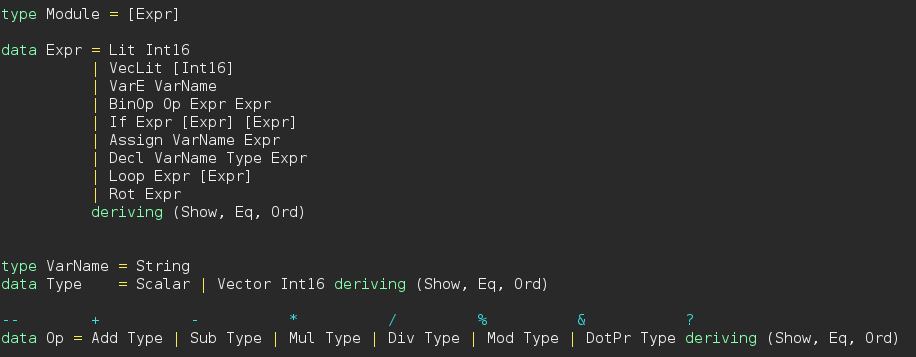
\includegraphics[scale=0.5]{images/AST.png}
    \caption{Abstrakcyjne drzewo syntaktyczne naszego języka w języku Haskell.}
    \label{fig:ast}
  \end{center}
\end{figure}

Omówimy teraz strukturę typu \texttt{Expr}, będącego centralnym typem dla naszego AST. Posiada on szereg konstruktorów, odpowiadających różnym elementom języka:
\begin{itemize}
  \item \texttt{Lit} -- literał, pojedyncza skalarna wartość. Choć język nie rozróżnia wektorów od skalarów, są one inaczej parsowane przez parser
  \item \texttt{VecLit} -- literał będący wektorem, czyli zapisany bezpośrednio w kodzie programu wektor
  \item \texttt{VarE} -- użycie zmiennej, pobranie z niej wartości do wykorzystania w wyrażeniu
  \item \texttt{BinOp} -- operacja binarna, niesie informacje o użytym operatorze (\texttt{+}, \texttt{-}, etc.) i operandach
  \item \texttt{If} -- wyrażenie warunkowe, zawierające dodatkowo jako pola warunek i listy wyrażeń wykonywanych w razie spełnienia warunku i w przeciwnym wypadku
  \item \texttt{Assign} -- przypisanie do zmiennej, niosące informację o nazwie zmiennej i wyrażeniu, które się pod nią podstawia
  \item \texttt{Decl} -- deklaracja zmiennej, będąca jednocześnie jej inicjalizacją. Dodatkowe pola to nazwa zmiennej, typ i wyrażenie inicjalizujące
  \item \texttt{Loop} -- pętla, pozwalająca na wykonanie określoną liczbę razy listy instrukcji
  \item \texttt{Rot} -- dedykowana instrukcja służąca rotowaniu czworokątów na płaszczyźnie
\end{itemize}

Studiując AST można zauważyć szereg decyzji dotyczących formy języka, na przykład: nie jest możliwe zadeklarowanie zmiennej bez jej inicjalizacji. Umożliwienie tego powoduje dużo błędów, gdy programista zapomni przypisać początkowych wartości do zmiennej i dostanie ona przypadkową wartość, która została w danej komórce pamięci. Takie błędy są stosunkowo trudne do wyśledzenia, a możliwość pominięcia inicjalizacji nie daje programiście w zamian wiele ekspresji. Utworzenie osobnej instrukcji \texttt{Rot} jest konsekwencją koncepcji procesora i języka: programista nie powinien operować ręcznie na adresach pamięci czy wręcz na pojedynczych elementach wektora. Powinien dostać gotowy, wspierany sprzętowo sposób osiągnięcia swojego celu.

\subsection{Lexer}

Lekser służy do podziału wejścia kompilatora na tokeny zgodnie z regułami podanymi przez twórcę języka. O tokenach możemy myśleć jako o najmniejszych, atomowych częściach języka. Lekser rozpoznaje również znaki specjalne i słowa kluczowe języka. Dzięki temu parser nie musi operować na ciągłym tekście, a skończonym zestawie tokenów, które dużo łatwiej przetwarzać, jako że znamy ich kategorie. Lekser został zaimplementowany przy użyciu popularnej biblioteki do parsingu napisanej w języku Haskell: Parsec. Więcej o tej bibliotece powiemy w kolejnym podpunkcie, dotyczącym parsera.

\subsection{Parser}

Parser służy do tłumaczenia tekstu programu na abstrakcyjne drzewo syntaktyczne. Najpopularniejszym podejściem przy tworzeniu parserów i lekserów jest ich generacja narzędziami takimi jak Lex, Yacc czy Bison, które dostawszy opis tokenów i gramatyki języka, są w stanie wyprodukować program parsera (zazwyczaj są to parsery LR lub pokrewne)[3]. Jakkolwiek dostajemy w ten sposób parsery bardzo wydajne, to taka technika jest niewygodna, wymaga znajomości specyficznej składni do zapisu tokenów i gramatyk, korzystania z dodatkowych narzędzi i utrudnia ewentualne zmiany w języku. Podejście, które wybrano przy tworzeniu projektu jest zgoła inne. Do języka Haskell dostępna jest dojrzała i stabilna biblioteka Parsec, oferująca monadyczne parsery działające na zasadzie tzw. \textit{parser combinators}. Są to rekurencyjne parsery top-down, które działają na zasadzie składania prostszych parserów w bardziej złożone. (Parser jest funkcją, która czyta wejście i zwraca parser, a zatem parsery bardziej skomplikowanych wyrażeń możemy składać z prostszych parserów).

Monadyczność jest pojęciem specyficznym dla programowania funkcyjnego i polega na używaniu do implementacji oprogramowania struktur nazywanych \textit{monadami}. Umożliwiają one między innymi osadzenie w języku funkcyjnym obliczeń, które mają efekty (w Haskellu monady są kluczowym pojęciem języka i wykorzystywane są do tak elementarnych operacji jak wejście-wyjście czy obsługa błędów).

\begin{figure}
  \begin{center}
    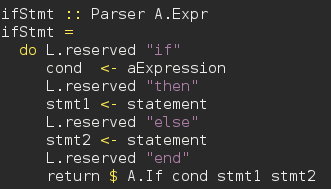
\includegraphics[scale=0.5]{images/parsing.png}
    \caption{Przykład zastosowania monadycznej składni do sparsowania wyrażenia warunkowego}
    \label{fig:parsing}
  \end{center}
\end{figure}

Monadyczny styl powoduje, że możemy napisać konstrukcję jak na rysunku \ref{fig:parsing}. Operator ,,\texttt{<-}'' jest charakterystyczną dla monad operacją \textit{bind}, która pozwala na wydobywanie wartości z monad z uwzględnieniem efektów, jakie były z daną wartością stowarzyszone. W tym przypadku mówimy parserowi, że aby sparsować wyrażenie warunkowe, musi najpierw znaleźć dopasowanie słowa kluczowego \texttt{if}, następnie spróbować sparsować warunek za pomocą parsera \texttt{aExpression} i nadać mu nazwę \texttt{cond} i wykonać podobne czynności dla kolejnych części instrukcji warunkowej. Ostatnia instrukcja na rysunku wykorzystuje operator \textit{return} by umieścić tworzony element drzewa AST (w tym przypadku jest to konstruktor \texttt{If} typu \texttt{Expr}, zawierający jako pola sparsowane przez nas elementy wyrażenia warunkowego) w monadycznym kontekście. Skojarzenie z instrukcją \texttt{return} z języków imperatywnych jest zupełnie niepoprawne, choć potrzeba czasu, by przestało się nasuwać --- \texttt{return} z Haskella nie wychodzi z funkcji, a ,,otacza'' zwykłą wartość monadą. Możemy zatem napisać \texttt{let a = return "Ala ma kota"} i w zmiennej \texttt{a} znajdzie się wartość typu \texttt{m String}, gdzie \texttt{m} jest dowolną, dedukowaną z kontekstu monadą.


\subsection{Instrukcje Assemblera}

Moduł \texttt{CodeGen.ASM} zawiera przede wszystkim opis mnemoników języka assembler, produkowanego przez kompilator oraz pomocnicze funkcje do tworzenia wartości w liczbowych w języku i konwersji mnemoników z abstrakcyjnych struktur na tekst, celem ich wyświetlenia. Poniżej znajduje się opis wszystkich instrukcji assemblera, zaimplementowanych w kompilatorze jako różne konstruktory jednego typu: \texttt{ASM}.

\begin{itemize}
  \item \texttt{Load addr} -- ładuje wartość spod podanego adresu (\texttt{addr}) w pamięci i wrzuca ją na stos
  \item \texttt{Store addr} -- odwrotność instrukcji \texttt{Load}, ściąga wartość ze szczytu stosu i zapisuje ją pod podany adres do pamięci
  \item \texttt{Push addr} -- wrzuca na stos stałą (przypomnijmy, że stałe trzymane są w osobnym segmentcie stałych, tak więc instrukcja \texttt{Push} przyjmuje nie cały wektor, a jedynie jego adres w tablicy stałych
  \item \texttt{MovS1} -- instrukcja specyficzna dla architektury z trzema stosami: ściąga wartość z głównego stosu i wrzuca na pierwszy stos pomocniczy
  \item \texttt{MovS2} -- podobnie do poprzedniej instrukcji, jednakże wrzuca na drugi stos pomocniczy
  \item \texttt{JumpZ lab} -- instrukcja skoku warunkowego, przeskakuje do wskazanej etykiety tylko, jeżeli na szczycie stosu jest wartość 0
  \item \texttt{Jump lab} -- instrukcja skoku bezwarunkowego, skacze do etykiety niezależnie od wartości na stosie
  \item \texttt{JumpIPZ ipVal} -- instrukcja skoku warunkowego skacząca do konkretnej wartości wskaźnika instrukcji (IP -- Instruction Pointer)
  \item \texttt{Jump ipVal} -- instrukcja skoku bezwarunkowego, skaczące do wartości wskaźnika instrukcji
  \item \texttt{Add, Sub, Mul, Div} -- instrukcje skalarnych operacji arytmetycznych, ściągają ze stosu dwa operandy, wykonują na nich odpowiednie działanie i wrzucają na stos wynik
  \item \texttt{AddS, SubS, MulS, DivS} -- instrukcje operacji arytmetycznych operujące na pomocniczych stosach. Po kolei ściągają ze szczytu obydwu stosów pomocniczych, wykonują działanie na tych dwóch wartościach i wrzucają wynik na główny stos, aż do momentu, kiedy stosy pomocnicze będą puste
  \item \texttt{RotS} -- instrukcja odpowiedzialna za rotację wektorów
  \item \texttt{DotPr} -- instrukcja licząca iloczyn skalarny dwóch wektorów z wierzchołka stosu i wrzucająca wynik na stos
  \item \texttt{ModS} -- ściąga ze stosu dwa wektory, liczy resztę z dzielenia każdego elementu pierwszego z nich przez odpowiedni element drugiego i wrzuca wynik z powrotem na stos
\end{itemize}

W szczególnej relacji pozostają ze sobą instrukcje \texttt{Jump}, \texttt{JumpZ}, \texttt{JumpIP} i \texttt{JumpIPZ}. Kompilacja skoków warunkowych odbywa się w trzech etapach:
\begin{itemize}
  \item kompilator, widząc instrukcję warunkową lub pętlę tworzy odpowiednie etykiety: na początku pętli i tuż za ciałem pętli. Dzięki temu możemy użyć instrukcji skoku bezwarunkowego do początku pętli za każdym razem, gdy wykonamy wszystkie instrukcje z jej wnętrza oraz skoku warunkowego na początku pętli, by w razie wyzerowania warunku pętli skoczyć poza pętlę (zauważmy, że uwzględnia to brzegowy przypadek pętli z zerową liczbą iteracji).
  \item po wygenerowaniu całego kodu assemblera numerujemy wszystkie instrukcje programu (mamy pewność, że ich ilość już się nie zmieni).
  \item każdą instrukcję skoku do etykiety przerabiamy na instrukcję skoku do numeru instrukcji stowarzyszonego z daną etykietą. Same etykiety nie są przy tym usuwane, a jedynie ingorowane przez procesor jak pusta instrukcja (w ten sposób unikamy konieczności ponownej numeracji linii po usunięciu etykiety).
\end{itemize}

Dzięki opisanym zabiegom procesor może utożsamić numer instrukcji z jej adresem w pamięci instrukcji (przypomnijmy, że instrukcje mają długość jednego bajtu, więc nie potrzeba żadnego przeliczania adresów, jeśli komórki pamięci mają również po jednym bajcie), a więc sprzętowa implementacja instrukcji skoku ulega znacznemu uproszczeniu.

\subsection{System sprawdzania poprawności typów -- Typechecker}

Jak zostało wspomniane, język jest statycznie typowany, co oznacza, że kompilator może stwierdzić poprawność programów w zakresie typów danych i zgłosić ewentualne błędy. Zaletą takiego podejścia jest ograniczenie ilości błędów w czasie wykonania programu. Dodatkowo, statyczne typowanie znacząco ułatwia refaktoring kodu oraz zmiany w programie. Wyobraźmy sobie funkcję zwracającą wartości typu $Int$, którą wykorzystujemy w wielu miejscach w programie. Załóżmy również, że mamy typ zespolony będący parą liczb typu $Double$. W języku dynamicznie typowanym zmieniając wartość zwracaną przez funkcję na taki typ musimy (ręcznie bądź z pomocą IDE) znaleźć wszystkie miejsca, w których wołana jest funkcja i odpowiednio zmienić logikę programu. Kompilator języka statycznie typowanego ostrzeże nas o każdym niedopasowaniu typów, również w przypadku, gdy przeoczymy użycie funkcji w innym pliku, nie pozwalając na kompilację błędnego programu.

System typów naszego języka jest z jednej strony celowo ograniczony jeśli chodzi o liczbę dostępnych typów (możemy operować tylko na wartościach całkowitych, skalarnych i wektorowych), a z drugiej strony wprowadza ciekawą funkcjonalność w postaci kontroli długości wektorów w czasie kompilacji. Jest to bardzo ograniczona implementacja tzw. ,,dependent typing'' (typów zależnych [od wartości]), czyli pomysłu na uzależnienie typu od wartości tego typu. Najczęściej podawanym w literaturze przypadkiem użycia typów zależnych są właśnie listy wraz z zakodowaną długością. Dzięki temu możemy w czasie kompilacji wykrywać takie błędy jak pobieranie głowy pustej listy, których programiści często nie zauważają w kodzie i które mogą się ujawnić dopiero po długim czasie działania programu. W naszym języku typy zależne służą do kontroli poprawności obliczeń na wektorach: dodawać/odejmować możemy tylko wektory o takich samych długościach, a iloczyn skalarny dwóch wektorów daje w wyniku skalar. Dzięki temu możemy być pewni, że w czasie działania programu użytkownik nie zostanie zaskoczony niespodziewanym błędem. Dodatkowo, deklaracja wektora wymaga podania jego długości. Zapobiega to kolejnemu częstemu przeoczeniu: w języku C możemy zadeklarować tablicę dziewiętnastu elementów i zainicjalizować ją tylko osiemnastoma. Wynik prostego błędu może spowodować trudne do wyśledzenia nieporządane zachowanie programu. Nasz język wymaga, by przy deklaracji wektora podać liczbę jego elementów i zainicjalizować go właśnie tyloma wartościami.

Sprawdzanie zgodności długości wektorów odbywa się poprzez rekurencyjną analizę operandów każdego wyrażenia wymagającego zgodności wymiarów (przypisanie i operacje arytmetyczne). Przykładowo, by sprawdzić zgodność wyrażenia binarnego staramy się wyinferować i porównoać liczbę elementów każdego z operandów. Jako że operandy same w sobie mogą być wyrażeniami, musimy sprawdzić również ich typ. W ten sposób przechodzimy całe drzewo AST, sprawdzając jego poprawność pod względem typów.

Aby implementować to i kolejne przejścia po AST z jednoczesnym zbieraniem informacji w pewnych strukturach i zgłaszaniem wyjątków, stosujemy jedną z zaawansowanych technik języka Haskell --- ,,\textit{monad transformers}''. Umożliwiają one połączenie funkcjonalności dwóch monad (zwykłe złożenie monad nie daje nam takich możliwości). Na rysunku \ref{fig:type-state} widzimy deklarację typu pozwalającego na odczyt i zapis do stanu skojarzonego z wyrażeniem za pomocą funkcji \texttt{get} i \texttt{put}, jak również przerywanie działania typecheckera za pomocą instrukcji \texttt{throwE}, działającej w sposób zbliżony do wyjątków w językach Java czy Scala. Jednocześnie nie tracimy żadnej z zalet programowania funkcyjnego, gdyż program nie łamie żadnego z jego założeń.

\begin{figure}
  \begin{center}
    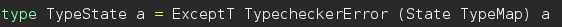
\includegraphics[scale=0.5]{images/type-state.png}
    \caption{Przykład zastosowania Monad Transformers do uzyskania struktury pozwalającej na przetrzymywanie stanu i rzucanie wyjątków bez wychodzenia poza czysto funkcyjny paradygmat.}
    \label{fig:type-state}
  \end{center}
\end{figure}

\subsection{Moduł konwersji wektorów -- Vectors}

Ten niewielki moduł jest istotnym elementem koncepcji procesora wektorowego. Odpowiada za podział wektorów na kawałki po osiem elementów (w przypadku, gdy długość wektora jest niepodzielna przez osiem, ostatni kawałek jest dopełniany zerami do pełnej ósemki -- w ten sposób zawsze operujemy na ośmioelementowych kawałkach (,,\textit{chunks}'') co pomaga w zaprojektowaniu procesora. Przykładowo, skalar \texttt{5} zostanie przerobiony na wektor \texttt{[0, 0, 0, 0, 0, 0, 0, 5]}, a dziesięcioelementowy wektor \texttt{[1, 2, 3, 4, 5, 6, 7, 8, 9, 10]} zostanie podzielony na dwa kawałki: \texttt{[0, 0, 0, 0, 0, 0, 0, 1, 2]} oraz \texttt{[3, 4, 5, 6, 7, 8, 9, 10]}. Kawałki są zaimplementowane jako osobny typ danych \texttt{Chunk}, dzięki czemu generator assemblera może traktować dowolny wektor jako listę kawałków (\texttt{[Chunk]}) i ich poprawność będzie statycznie sprawdzana.

Moduł \texttt{Vectors} udostępnia funkcje do konwersji skalarów na wektory oraz podziału długich wektorów na kawałki -- w ten sposób wynikowy kod assemblera nigdy nie zawiera skalarów ani wektorów o niespodziewanych długościach.


\subsection{Generator kodu assemblera}

Jeden z głównych (obok Parsera) modułów kompilatora, odpowiedzialny za generację kodu assemblera na podstawie abstrakcyjnego drzewa syntaktycznego. W zarysie idea polega na przejściu całego drzewa AST i generacji assemblera dla każdego napotykanego węzła w drzewie. Proces ten rekurencyjnie zagłębia się w złożone struktury, generując assembler dla podwyrażeń. Przykładowo, chcąc wygenerować kod dla operacji binarnej musimy najpierw wygenerować kody dla wyliczenia obydwu jej operandów i użyć ich do odpowiedniego skonstruowania ostatecznego kodu instrukcji. Język Haskell wyjątkowo dobrze nadaje się do tego typu operacji, udostępniając programiście omawiane już algebraiczne typy danych (,,algebraic datatypes''), na których z łatwością możemy stosować tzw. ,,pattern matching'', czyli dopasowywanie konstruktora typu do wzorca, używane przy deklaracji funkcji i wyrażeniach warunkowych \texttt{case}. Dzięki temu ułatwione jest trawersowanie drzew: w każdym węźle możemy wykonać ,,\textit{pattern matching}'' i dopasować podejmowane działania w zależności od rodzaju liścia. Przyjrzyjmy się funkcji przetwarzającej na kod assemblera pojedyncze wyrażenie (\texttt{Expr}), widocznej na rysunku \ref{fig:processExpr}.

\begin{figure}
  \begin{center}
    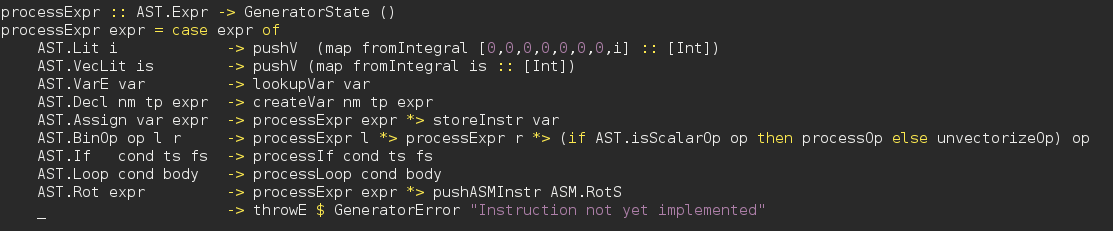
\includegraphics[scale=0.5]{images/processExpr.png}
    \caption{Przykład zastosowania pattern matchingu do przetwarzania typu danych z wieloma konstruktorami.}
    \label{fig:processExpr}
  \end{center}
\end{figure}

Kolejnym ciekawym mechanizmem zastosowanym w omawianym przykładzie jest użycie tzw. aplikatywów (,,applicatives''), będących nieco mniej ekspresyjną wersją monad. Udostępniają możliwość wykonywania sekwencyjnie obliczeń i umieszczania ich w pewnym kontekście, ale nie dają tak wielu funkcjonalności i nie mają tak rozwiniętej syntaktyki jak monady. W powyższym przykładzie ich użycie sprowadza się do użycia operatora \texttt{*>}, wykonującego swój prawy operand i zwracającego wartość lewego operandu. Warto zaznaczyć, że, podobnie jak w przypadku monad, zyskujemy możliwość sekwencyjnego wykonywania akcji, a nie tracimy żadnej z zalet programowania funkcyjnego.

W nowych wersjach Haskella (od 7.10 w górę) każda monada jest równocześnie aplikatywem, ale nie na odwrót.

Działanie generatora nie ogranicza się do prostego przetwarzania każdego wyrażenia. Dzięki użyciu podobnego zabiegu, jak w przypadku Typecheckera, rekurencyjne trawersowanie po drzewie odbywa się przy towarzyszeniu stanu, w którym przetrzymywane są informacje o bieżącym stanie generacji. Są to w szczególności: wygenerowany do tej pory assembler, dane o przypisaniu stałych w tablicy stałych, całość AST, które przetwarzamy (pozwala nam się to odnosić globalnie do całości drzewa przy przetwarzaniu poszczególnych instrukcji; w przeciwnym razie każde rekurencyjne zejście pozbawia nas informacji o ,,korzeniach'' drzewa, której być może będziemy potrzebować do analizy bardziej złożonych instrukcji), tablica symboli, czyli przypisania do nazw zmiennych informacji o nich, informacja o dostępnych adresach alokacji zmiennych w pamięci i dostępne etykiety do skoków. Całość tej informacji trzymana jest w jednym typie danych: \texttt{GeneratorData}, którego budowa przedstawiona jest na rysunku \ref{fig:generator-data}.

\begin{figure}
  \begin{center}
    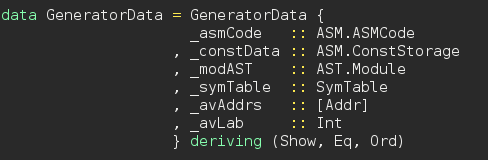
\includegraphics[scale=0.5]{images/generator-data.png}
    \caption{Struktura danych do przechowywania informacji o stanie generacji kodu assemblera wraz z towarzyszącymi strukturami.}
    \label{fig:generator-data}
  \end{center}
\end{figure}

Oprócz tego, Generator używa wielu pomocniczych funkcji w celu sprawdzania adresów, które przypisuje zmiennym, wyszukiwania informacji zmiennych w mapie -- tablicy symboli, sprawdzania długości wektorów, konwersji pętli i instrukcji warunkowych na logikę używającą skoków warunkowych i bezwarunkowych oraz wielu innych. Dodatkowo, zawiera kod obsługujący błędy czasu kompilacji za pomocą zgłaszania wyjątków. Podobnie jak przy typecheckingu jest to możliwe w elegancki i czysto funkcyjny sposób dzięki zastosowaniu \textit{monad transformers}.

Reasumując, Generator jest jednym z najbardziej rozbudowanych modułów kompilatora i używa wielu zaawansowanych technik języka Haskell. Dzięki temu możliwe było napisanie go w zwięzły, niezawodny i przejrzysty sposób, bez jednoczesnego poświęcania wygody tworzenia oprogramowania. Jest to jeden z modułów, w którym dobitnie przejawia się sensowność użycia języka Haskell jako głównej technologii przy tworzeniu kompilatora.

\subsection{Moduł konwersji etykiet -- LabelRename}

Moduł ten służy do opisanego już zamieniania skoków do etykiet na skoki do konkretnych adresów instrukcji. By możliwe było to w łatwy sposób do assemblera zostały wprowadzone dwie dodatkowe instrukcje: obok \texttt{Jump} (instrukcja skoku) i \texttt{JumpZ} (instrukcja skoku warunkowego), mamy także \texttt{JumpIP} i \texttt{JumpIPZ}, które mają analogiczną semantykę, ale zamiast skakać do etykiet, skaczą do konkretnych wartości wskaźnika instrukcji (\textit{Instruction Pointer} -- IP). W przyjętej przez nas architekturze procesora, w szczególności przy jednobajtowych instrukcjach i osobnej pamięci instrukcji, wartość wskaźnika instrukcji jest tożsama z adresem w pamięci odpowiadającej mu instrukcji. Dzięki takim zabiegom możliwe jest zrealizowanie konwersji skoków w relatywnie nieskomplikowany sposób:

\begin{itemize}
  \item dla każdej instrukcji warunkowej (\texttt{if}) i każdej pętli (\texttt{loop}), generujemy odpowiednie etykiety i skoki do nich
  \item po wygenerowaniu całego kodu assemblera numerujemy linie (będą to przyszłe adresy instrukcji w pamięci)
  \item przeglądamy po kolei instrukcje i jeśli znajdziemy etykietę pobieramy jej numer linii; następnie znajdujemy wszystkie instrukcje skoku do tej etykiety i zamieniamy je na instrukcje skoku do wskaźnika instrukcji, podając pobrany numer linii jako argument
\end{itemize}

W ten sposób nasz kod assemblera nie zawiera już odniesień do etykiet, a jedynie instrukcje zrozumiałe dla procesora, każące mu jako następną przetwarzaną instrukcję załadować instrukcję spod określonego adresu w pamięci. Warto zwrócić uwagę, że etykiety nie są usuwane, a będą pomijane przez procesor --- wykonanie jednej dodatkowej, pustej instrukcji dla każdej instrukcji ma zaniedbywalny koszt podczas wykonania programu (zajmuje to 3 cykle zegara), a uproszczenie konwersji etykiet jest znaczące: nie musimy przenumerowywać instrukcji, co podniosłoby złożoność algorytmu. Proces jest dość kosztowny czasowo, jako że jego złożoność czasowa to $\mathcal{O}(n^2)$, gdzie n jest liczbą instrukcji assemblera, ale nie ma to większego wpływu na wydajność całego procesu kompilacji, gdyż w porównaniu z generacją assemblera czy parsingiem będzie to zawsze niewielka wartość (liczba instrukcji powstająca w wyniku kompilacji jest dla tej architektury stosunkowo niewielka). Dodatkowo, takie przetworzenie etykiet znacząco upraszcza działanie układu przetwarzającego instrukcje w procesorze.


\subsection{Moduł binaryzacji assemblera -- Binary}

Ostatni etap kompilacji, polegający na konwersji instrukcji assemblera (zapisanych jako typy danych języka Haskell, ale posiadających również czytelną reprezentację tekstową) na postać binarną, gotową do wysłania przez port szeregowy do procesora. Decyzje podjęte podczas projektowania protokołu binaryzacji mają duży wpływ na obsługę transmisji i dekodowania instrukcji w procesorze. Początkowa koncepcja zakładała przesyłanie jednobajtowych instrukcji z wielobajtowymi operandami (m.in. z wektorami zapisanymi jako operandy instrukcji push). Po konsultacjach uznano, że najkorzystinejsza forma instrukcji to instrukcje o stałej, jak najmniejszej liczbie bajtów. Instrukcję \texttt{Push} przerobiono tak, by zamiast przetrzymywać stałe programu jako operandy, odczytywała jest z tablicy stałych, a jako operand przetrzymywała jedynie adres w tej tablicy. Pozostawał jeszcze problem z instrukcjami skoku, które posiadają sześciobajtowy adres jako argument. Istniała obawa, ze instrukcje będą musiały mieć dwa bajty: po jednym na instrukcję i jej argumenty. Okazało się jednak, że dzięki zastosowaniu bezprefiksowego kodowania instrukcji jesteśmy w stanie zmieścić wszystkie instrukcje wraz z argumentami na jednym bajcie, co przyniosło wiele korzyści.

Bezprefiksowe kodowanie oznacza, że żadna instrukcja nie może być przedrostkiem innej instrukcji. Dzięki temu możemy zakodować instrukcje skoku jako posiadające najstarszy bajt ustawiony na 1, a resztę bajtów przeznaczyć na adres. Inne instrukcje, dla których bajty 2-8 będą nie adresem, a częścią instrukcji, muszą mieć pierwszy bajt ustawiony na 0. Dzięki temu uzyskujemy optymalne wykorzystanie dostępnej przestrzeni kodowań i brak niejednoznaczności.

\section{FPGA}

Koprocesor został zaimplementowany na układzie FPGA, a do opisu sprzętu użyto języka VHDL (Very High Speed Integrated Circuits Hardware Description Language)[5]. Jako dostawcę płytek wybrano firmę Altera --- projekt był testowany na zestawie uruchomieniowym Altera De0-nano[6]. Jest to niewielka, edukacyjna płytka, która mimo to posiada stosunkowo współczesny układ FPGA Cyclone IV. Oprócz tego, płytka posiada dużą ilość pinów GPIO (\textit{General Purpose Input/Output} -- wejście/wyjście ogólnego przeznaczenia), z których możemy korzystać do podłączania rozmaitych urządzeń peryferyjnych, jak w naszym przypadku przewodów transmisji UART.

\begin{figure}
  \begin{center}
    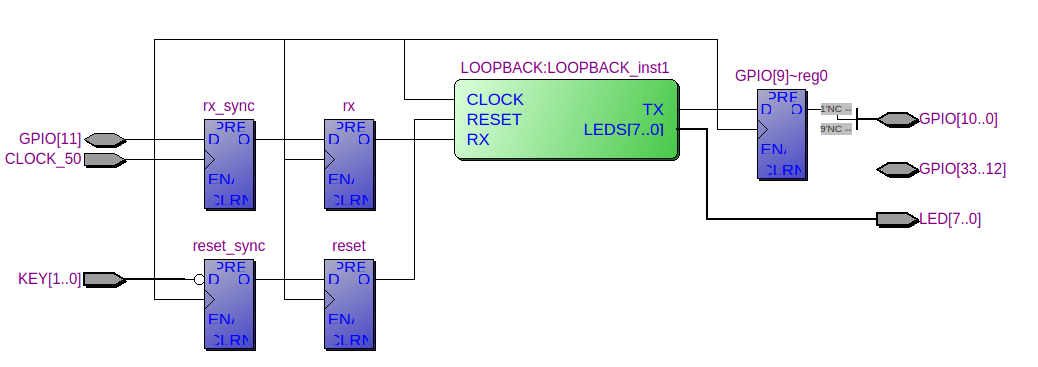
\includegraphics[scale=0.5]{images/schemat.png}
    \caption{Przeglądowy schemat wyprowadzeń układu. Schemat komponentu loopback, choć dużo ciekawszy, jest zbyt złożony, by w całości przedstawić go na jednym rysunku (jest na nim prawie pięć tysięcy elementów).}
    \label{fig:schemat}
  \end{center}
\end{figure}

Do tworzenia projektu na FPGA użyto dedykowanego do układów Altery środowiska Quartus II, które dostarcza pełny zestaw narzędzi do tworzenia i testowania projektów FPGA. Quartus posiada przede wszystkim zaawansowany kompilator, syntezator i \textit{fitter}, które potrafią z opisu w języku VHDL utworzyć fizyczny rozkład bramek na płytce. Jest to wysoce nietrywialne zadanie, jako że muszą one najpierw stworzyć na podstawie opisu poprawny układ elektroniczny, a następnie wielokrotnie go optymalizować tak, by spełnił wymagania czasowe, napięciowe oraz przestrzenne. Istotnym parametrem syntezy i \textit{fittingu} jest ukierunkowanie na szybkość układu lub niską liczbę bramek (są to wzajemnie wykluczające się wartości). Do budowania projektu używano ustawień nastawionych na jak największą szybkość: kompletny układ zajmuje około 4500 elementów logicznych, czyli 25\% zasobów płytki. Z tego powodu można było sobie pozwolić na optymalizację pod kątem czasu działania.

W następnych akapitach opisane zostaną główne komponenty wchodzące w skład koprocesora. Każdy z nich jest osobną jednostką (\textit{entity}) języka VHDL.


\subsection{Główny moduł}

Znajduje się w pliku \texttt{fpga\_coprocessor.vhd}. Służy głównie do zainstancjonowania głównej maszyny stanów procesora i podłączenia jej do zewnętrznego świata. W tym module znajdują się deklaracje pinów odpowiadających fizycznym pinom na płytce. Aby zapewnić lepsze działanie wejścia/wyjścia, sygnały wejściowe (tj. reset i sygnał z pinu RX) są synchronizowane kaskadowo na dwóch rejestrach. Jest to praktyka polecana przez Alterę i sugerowana jako ostrzeżenie czasu kompilacji, gdy nie jest stosowana. Zamiast, żeby reset był asynchroniczny, jest przypisywany w synchronizowanym zegarem procesie do jakiegoś rejestru, którego wartość jest w tym samym procesie przypisywana do kolejnego rejestru. Dopiero z tego ostatniego rejestru czytamy wartość sygnału i dalej ją przetwarzamy. Dzięki temu unikamy nieporządanych zachowań układu, które mogłyby na przykład spowodować, że maszyna stanów będzie się zachowywać niedeterministycznie.


\subsection{Główna maszyna stanów}

Znajduje się w pliku \texttt{loopback.vhd}. Nazwa loopback ma uzasadnienie po części historyczne, a po części merytoryczne. Podczas testów różnych implementacji transmisji szeregowej moduł loopback wykorzystywany był, by sprawdzić działanie transmisji na najprostszym możliwym przykładzie, tj. układzie odsyłającym wszystko to, co zostało do niego wysłane. Dodatkowo, cały procesor działa obecnie na nieco podobnej zasadzie: otrzymuje dane i program i odsyła dane. Jest więc w pewnym sensie rozwinięciem koncepcji loopback[7].

Moduł \texttt{loopback} to najważniejszy i najbardziej złożony moduł koprocesora. Jego główną część stanowi maszyna stanów, która reaguje na przychodzące od strony komputera dane, a następnie zaczyna wykonywać otrzymany program. Po wykonaniu ostatniej instrukcji maszyna stanów zaczyna inicjować odsyłanie danych do komputera. Co ważne, cała maszyna jest synchronizowana zegarem (alternatywnie, można skonstruować maszynę, w której synchronizowany zegarem jest tylko proces zmieniający stan maszyny na kolejny, a proces realizujący przejścia między stanami jest wzbudzany zmianą stanu). Altera w swojej dokumentacji zachęca do stosowania synchronicznych układów, jako że są one bardziej deterministyczne i dają mniej problemów z czasami propagacji. Intuicyjnie: jeśli układ jest synchroniczny, to stan logiczny sygnałów zmienia się w takt zmian sygnału zegara. Jeśli zaś zaczniemy tworzyć układ asynchroniczny, powodujemy powstanie długich ścieżek, na których czasy propagacji mogą zacząć się sumować do nieakceptowalnych wartości. Dodatkowo, przy synchronizacji całej maszyny stanów jednym zegarem unikamy problemów przy podłączaniu do niej komponentów synchronizowanych zegarem. Na rysunku \ref{fig:PSM} znajduje się diagram stanów omawianej maszyny. 

\begin{figure}
  \begin{center}
    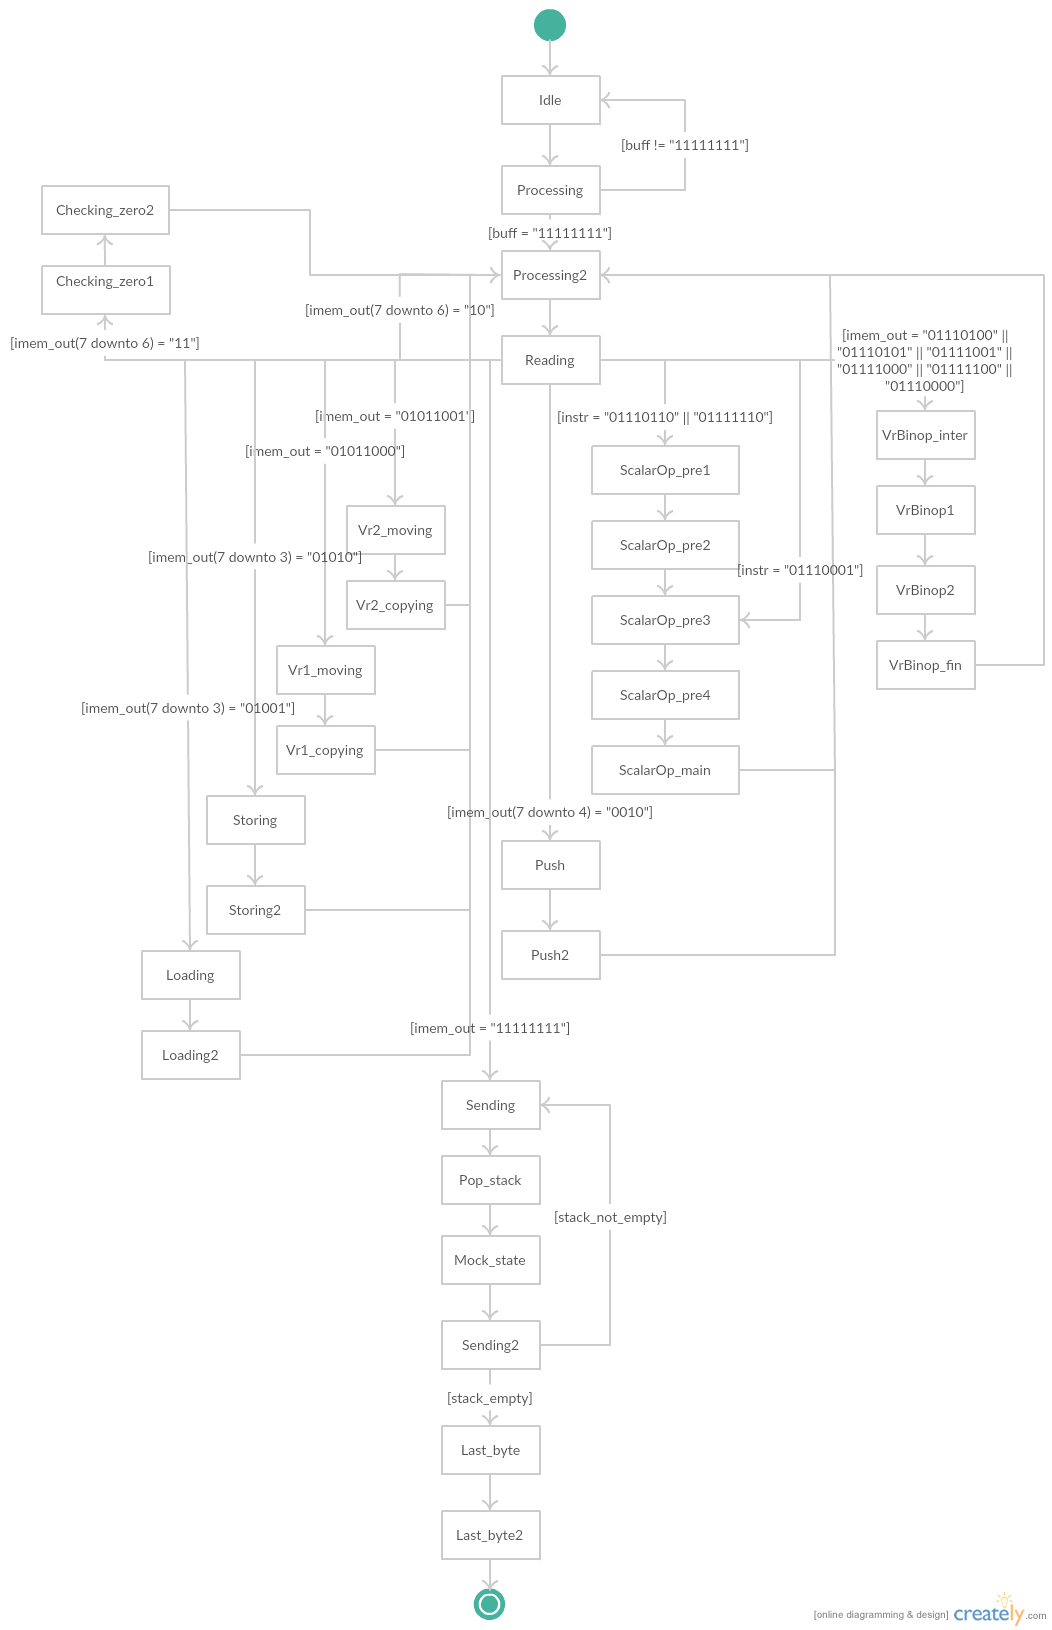
\includegraphics[scale=0.4]{images/Processor-State-Machine.png}
    \caption{Diagram maszyny stanów procesora. W nawiasach kwadratowych znajdują się zdarzenia warunkujące przejście do konkretnego stanu. Brak adnotacji przy strzałce oznacza przejście bezwarunkowe.}
    \label{fig:PSM}
  \end{center}
\end{figure}

Na rysunku widać podział maszyny na trzy części, na diagramie ułożone od góry do dołu. Pierwsza z nich to stany \texttt{Idle} i \texttt{Processing}, które odpowiadają za odbieranie ciągu instrukcji i danych od procesora. Następnie widzimy dużą grupę zapętlających się stanów, krążących między stanami \texttt{Reading} i \texttt{Processing2}, stanowiących główną pętlę odczytującą i wykonującą instrukcje programu. Ostatnia część to cztery instrukcje na samym dole, odpowiedzialne za odesłanie danych do komputera. Opiszemy teraz z większą dokładnością ważniejsze stany/grupy stanów maszyny:

\begin{itemize}
  \item \texttt{Idle} -- procesor czekający na dane. Dzięki konstrukcji maszyny stanów możemy w tym stanie umieścić instrukcję \texttt{if} czekającą, aż zapalona zostanie flaga świadcząca, że coś jest odebrane przez interfejs UART. Wtedy dopiero wykonujemy odpowiednią operację (zapisujemy bajt, który przyszedł albo do pamięci instrukcji, albo do pamięci stałych) i możemy przejść do stanu \texttt{Processing}. To, czy wybierzemy pamięć instrukcji, czy pamięć stałych zależy od wartości flagi, którą ustawiamy w stanie \texttt{Processing}.
  \item \texttt{Processing} -- druga część pętli odbierającej dane. Potrzebne jest rozdzielenie odbierania danych na co najmniej dwa stany, jako że zapis do pamięci zajmuje dwa cykle (ustawiamy adres i wartość do zapisania w pamięci i w kolejnym cyklu sygnały odpowiednio się ustalają). W stanie \texttt{Processing} sprawdzamy, czy to, co przyszło, nie było bajtem złożonym z samych jedynek (\texttt{"11111111"}). Jeśli tak, to zapalamy flagę świadczącą o zakończeniu odbierania instrukcji i rozpoczęciu odbierania danych (w każdym programie ciąg instrukcji zakończony jest bajtem samych jedynek; następnie mamy po osiem bajtów stałych i na koniec segmentu stałych kolejny bajt samych jedynek). Jeśli bajt jedynek pojawił się po raz drugi, będziemy przechodzili w stan \texttt{Processing2} zamiast \texttt{Idle}.
  \item \texttt{Processing2} -- stan przejściowy przed stanem \texttt{Reading}. Jego główną funkcją jest odczekanie jednego cyklu celem ustalenia się wartości syngałów, przede wszystkim w pamięciach, oraz wyzerowanie wszystkich flag uruchamiających zapis do pamięci.
  \item \texttt{Reading} -- największy stan maszyny. Składa się z wielkiego wyrażenia warunkowego, które sprawdza instrukcję znajdującą się pod obecnym adresem w pamięci instrukcji. Zależnie od kadu instrukcji wykonywane są przejścia do odpowiednich stanów i modyfikowane są flagi oraz adresy pamięci. Na rysunku \ref{fig:PSM} znajduje się dokładny opis przejść.
  \item \texttt{Loading} (wraz z towarzyszącym mu \texttt{Loading2}) -- w \texttt{Reading} został ustawiony odpowiedni adres pamięci RAM, w \texttt{Loading} odczytana zostanie wartość z pamięci i zostanie wrzucona na stos. \texttt{Loading2} dostarcza dodatkowy cykl potrzebny na ustalenie się stanów logicznych w procesach. Dokładny sposób działania stosu i pamięci RAM zostanie opisany przy opisie tych komponentów.
  \item \texttt{Storing} (wraz ze \texttt{Storing2}) -- odwrotnie do \texttt{Loading}, wartość jest najpierw pobierana ze stosu (\texttt{pop}), a następnie zapisywana do pamięci.
  \item \texttt{VrMoving, VrMopying} w wersjach dla pierwszego i drugiego stosu pomocniczego -- sekwencja moving i copying spowoduje, że wartość z głównego stosu zostanie ściągnięta i wrzucona na odpowiedni stos pomocniczy.
  \item \texttt{Push} i \texttt{Push2} -- część instrukcji polegająca na odczytaniu stałej spod odpowiedniego adresu w pamięci stałych wykonywana jest już w stanie \texttt{Reading} podczas dekodowania instrukcji. Pozostaje poczekać, aż wartość się pojawi i wrzucić ją na stos.
  \item \texttt{ScalarOp} -- grupa pięciu instrukcji, które wykonują operacje na skalarach (czyli w efekcie na pojedynczych kawałkach wektora). Kolejne kroki to ściągnięcie pierwszej wartości ze stosu, ściągnięcie drugiej wartości ze stosu, wykonanie operacji i wrzucenie wyniku z powrotem na stos. W przypadku operacji unarnej skaczemy od razu do stanu ściągającego drugą wartość ze stosu, dzięki czemu pobierany jest tylko jeden operand.
  \item \texttt{VrBinop} -- operacje wektorowe, których działanie jest kluczowe dla działania procesora. Jeśli wykonujemy binarną operację wektorową dzieją się następujące kroki: wszystkie kawałki pierwszego operandu są przerzucane na pierwszy stos pomocniczy, wszystkie kawałki drugiego operandu są przerzucane na drugi stos pomocniczy. Następnie po kolei ściągamy po jednym kawałku ze stosu pierwszego i drugiego, wykonujemy operację binarną na dwóch kawałkach i wynik wrzucamy na główny stos. Powtarzamy ściąganie i operację aż do momentu, w którym stosy pomocnicze będą puste. Zauważmy, że w ten sposób na stosie głównym znajduje się wektor, który ma oryginalną kolejność kawałków (wrzucanie na stos po kolei odwraca kolejność, ale zostało wykonane dwukrotnie).
  \item \texttt{Sending} -- stan inicjujący odsyłanie danych. Odsyłana jest cała zawartość stosu, jako że po wykonaniu programu maszyny stosowej na stosie powinna zostać pojedyncza wartość, złożona ewentualnie z wielu kawałków.
  \item \texttt{PopStack} -- jak sama nazwa wskazuje, w tym stanie zdejmowana jest wartość ze stosu i stan zmieniany jest na \texttt{MockState}.
  \item \texttt{MockState} -- nazwa została z powodów historycznych, jako że pierwotnie stan ten służył jedynie ustaleniu się wartości odczytanej ze stosu. Obecnie służy do obsługi bufora wyjścia (UART wysyła po bajcie, a wartości na stosie mają osiem bajtów. Utworzony jest więc bufor, do którego zapisywana jest wartość ze stosu, a który następnie jest po bajcie odsyłany do komputera) i dekrementacji licznika bajtów bufora pozostałych do wysłania.
  \item \texttt{Sending2} -- czeka, aż UART potwierdzi wysłanie bajtów i podejmuje szereg decyzji. Jeśli nie został wysłany cały bufor, wraca do stanu \texttt{MockState}. Jeśli bufor został wysłany, ale stos jeszcze nie jest pusty, wraca do stanu \texttt{Sending}. Jeśli stos jest pusty przechodzi do stanu \texttt{LastByte}.
  \item \texttt{LastByte} i \texttt{LastByte2} -- odpowiedzialne za wysłanie kończącego bajtu złożonego z samych jedynek. Dzięki temu program odbierający dane wie, że należy zakończyć transmisję.
\end{itemize}

\subsection{Stos}

Stosy używane są w programie w trzech miejscach (główny stos i dwa stosy pomocnicze do operacji wektorowych), jednakże są instancjami tej samej \textit{entity}, znajdującej się w pliku \texttt{stack.vhdl}. Stos działa na prostej zasadzie: oparty jest o pamięć, będącą tablicą ośmiobajtowych wektorów i wskaźnik stosu, który mówi nam, gdzie obecnie znajduje się wierzchołek stosu. Wybrana wersja stosu to stos rosnący w kierunku malejących adresów, ze wskaźnikiem stosu wskazującym pierwsze wolne miejsce do zapisu elementu. Alternatywnie stos mógłby rosnąć w kierunku rosnących adresu, a wskaźnik stosu wskazywać pierwszy element na stosie. Funkcjonalność stosu pozostaje niezmieniona po wybraniu innego podejścia do obsługi wskaźnika stosu, ale podejście zastosowane przez nas jest z powodzeniem stosowane w dużej ilości implementacji[4].

Stos posiada dwie istotne flagi: \texttt{enable} oraz \texttt{command}. Pierwsza z nich uruchamia stos, który dopiero gdy jest ona zapalona będzie analizował kolejną z flag (gdybyśmy nie mieli takiej flagi, to stos cały czas wykonywałby ostatnio wykonaną operację, czyli albo zapełniłby się cały jedną wartością, albo całkowicie opróżnił, jako że wejście do procesu kontrolującego stos następuje przy każdym zboczu rosnącym sygnału zegarowego). Flaga \texttt{command} mówi o rodzaju operacji, jaką należy wykonać na stosie, czyli \texttt{push} lub \texttt{pop}. A zatem wrzucanie elementu na stos odbywa się za pomocą następującej sekwencji działań:

\begin{itemize}
  \item ustawiamy flagę \texttt{enable} na \texttt{'1'}, flagę \texttt{command} na \texttt{'0'} i zapisujemy do wektora \texttt{push\_data} dane, które chcemy umieścić na stosie
  \item odczekujemy jeden cykl, aby sygnały zdążyły się ustalić (wartość z \texttt{push\_data} musi zostać przekopiowana, a wartość wskaźnika stosu musi zostać dekrementowana.
\end{itemize}

Podobnie przebiega odczyt ze stosu:
\begin{itemize}
  \item ustawiamy flagę \texttt{enable} na \texttt{'1'}, flagę \texttt{command} na \texttt{'1'}
  \item w kolejnym cyklu przypisujemy wartość \texttt{pop\_data} do docelowego bufora
  \item dopiero w następnym cyklu wartość w buforze jest ustalona
\end{itemize}

Warto zwrócić uwagę, że zapis na stos zajmuje dwa cykle zegara, a odczyt trzy i należy to wziąć pod uwagę podczas obsługi stosu w maszynie stanów. Podczas tworzenia projektu podobne niedopatrzenia były źródłem wielu problemów, które skutkowały niedeterministycznym zachowaniem układu. Stos operuje na ośmiobajtowych wektorach, reprezentujących jeden ,,kawałek'' (\textit{Chunk}) w nomenklaturze kompilatora. Dzięki temu \texttt{push} i \texttt{pop} są operacjami atomowymi dla ośmioelementowych kawałków wektorów.

Stos jest tak zaimplementowany, by Quartus inferował tablicę wektorów, do której zapisywane są wartości, jako pamięć RAM i zamiast elementów logicznych używał do tego statycznej pamięci RAM dostępnej na płytce. Powoduje to dużą oszczędność zasobów, tym bardziej, że na płytce mamy dostępne zaledwie 

\subsection{Pamięć RAM}

Pamięć RAM, podobnie jak stos, operuje na ośmiobajtowych wektorach. Wejścia komponentu to flaga \texttt{write\_enable} oraz adresy zapisu i odczytu. Odczyt dostępny jest zawsze, bo w żaden sposób nie ingeruje w zawartość pamięci. Aby odczytać wartość wystarczy ustawić adres odczytu, a po odczekaniu jednego cyklu pobrać wartość z wyjścia pamięci. Aby zapisać wartość należy ustawić flagę \texttt{write\_enable} i odpowiedni adres zapisu. W kolejnym cyklu należy wkopiować do wejścia pamięci wartość, którą chcemy zapisać. W następnym cyklu wartość będzie zapisana w pamięci. Ten sposób obsługi pamięci nie pozwala na sytuację jednoczesnego zapisu i odczytu. Nie jest to dla nas problemem, gdyż w naszym koprocesorze taka sytuacja nigdy nie może mieć miejsca.

Ilość cykli potrzebnych do operacji na pamięci jest odwrotna niż w przypadku stosu: zapis zajmuje trzy cykle, a odczyt jedynie 2. Tutaj również zapis i odczyt są operacjami atomowymi dla ośmioelementowych wektorów.


\subsection{Pamięć instrukcji}

Działa na identycznej zasadzie jak pamięć RAM (wewnętrznie jest pamięcią RAM, ale wprowadzamy nazwę ,,pamięć instrukcji'' dla rozróżnienia jej od pozostałych pamięci). Różnicą jest jedynie długość adresu (sześć bajtów) i operowanie na pojedynczych bajtach, zamiast na ośmioelementowych wektorach. Pamięć instrukcji jest liniowo zapełniana podczas odbierania instrukcji przez UART, a podczas działania procesora układ interpretujący instrukcje pobiera z niej po bajcie spod adresu wskazywanego przez aktualną wartość wskaźnika instrukcji.


\subsection{Pamięć stałych}

Pamięć stałych działa w nieco inny sposób niż pamięć RAM i pamięć instrukcji. Struktura jest dość podobna (mamy flagę \texttt{write\_enable}, bufor zapisu i odczytu oraz adres zapisu i adres odczytu), jednak zapis i odczyt nie są symetryczne, jak w poprzednim przypadku. Do pamięci zapisujemy po bajcie, jako że stałe do zapisania przychodzą przez port szeregowy po bajcie. Odczyt natomiast jest w kawałkach ośmioelementowych, gdyż procesor operuje tylko na takich wartościach. Taka asymetria powoduje, że z jednej strony używanie tej pamięci w maszynie stanów procesora jest niezwykle łatwe (nie trzeba manualnie przeliczać adresów ani iterować po bajtach), ale ma swoje konsekwencje: kompilator nie potrafi (nie jest to możliwe) wyinferować statycznej pamięci RAM, więc tracimy nieco zasobów płytki. Nie jest to jednak w żadnej mierze problemem, jako że nie brakuje zasobów na płytce, a projekt procesora sam w sobie jest bardzo kompaktowy.


\subsection{ALU}

Jednostka arytmetyczno-logiczna (\textit{Arithmetic-Logic Unit} -- ALU), odpowiadająca za wykonywanie działań na ośmioelementowych kawałkach wektorów. Każde z działań wykonywane jest w jednym cyklu zegara (ściśle mówiąc, logika ALU jako jedynej jednostki w projekcie nie jest synchroniczna; natura wykonywanych operacji pozwala je zaimplementować jako kombinacyjne funkcje wejść, co nie wprowadza takich opóźnień jak sekwencyjne przetwarzanie stanów, działająć natychmiast).

Operacje wykonywane przez ALU to:
\begin{itemize}
  \item suma -- nowy wektor powstaje przez dodanie odpowiadających sobie elementów wektorów wejściowych
  \item różnica -- jak w przypadku sumy, tylko dla odejmowania
  \item mnożenie \textit{element-wise} -- nowy wektor powstaje przez wymnożenie ze sobą odpowiednich elementów wektorów wejściowych (nie mylić z iloczynem skalarnym wektorów)
  \item dzielenie -- analogicznie do mnożenia \textit{element-wise}
  \item modulo -- każdy i-ty element wektora wyjściowego powstaje przez wyliczenie reszty z dzielenia i-tego elementu pierwszego operandu przez i-ty element drugiego operandu
  \item iloczyn skalarny -- dla wektorów $u$ i $v$ ich iloczyn skalarny wyliczamy jako $u \circ v = \sum_{i=1}^{\|u\|} v_i u_i $
  \item rotacja -- przyjmuje ośmioelementowy wektor, reprezentujący cztery punkty w dwuwymiarowej przestrzeni i obraca go względem punktu $(255, 255)$
\end{itemize}

\subsection{UART}

Obsługa portu szeregowego została zaimplementowana z wykorzystaniem modułu UART autorstwa Petera Benetta (https://github.com/pabennett)[8]. Z dostępnych publicznie implementacji ta wydaje się najstaranniej napisana i w naszych testach dawała zdecydowanie najlepsze wyniki. Obsługa modułu wymaga jednak pewnej uwagi, gdyż pomyłka o jeden cykl może spowodować zupełnie niespodziewane zachowanie transmisji. Moduł posiada dwa interfejsy: pierwszy, fizyczny, to po prostu dwa przewody: RX i TX, które wystarczy podłączyć do pinów GPIO na płytce. Ich obsługą zajmuje się sam moduł UART i korzystający z niego nie musi się tym zajmować. Drugi interfejs jest ,,wewnętrzny'', co oznacza, że korzystać z niego będzie maszyna stanów procesora by odbierać i wysyłać dane[9].

Aby wysłać bajt danych przez interfejs UART należy wykonać następującą sekwencję czynności:
\begin{itemize}
  \item załadować bajt do bufora wyjściowego
  \item ustawić flagę powodującą rozpoczęcie transmisji
  \item poczekać, aż ustawiona zostanie flaga potwierdzająca wysłanie całego bajtu
  \item w tym samym cyklu, w którym odczytaliśmy potwierdzenie wysłania należy wyłączyć flagę transmisji (w przeciwnym razie układ zacznie wysyłać kolejny bajt)
\end{itemize}

Aby odebrać bajt sekwencja wygląda następująco:
\begin{itemize}
  \item czekamy na ustawienie flagi informującej o przyjściu nowej wartości do bufora odbiornika
  \item gdy zostanie zapalona wspomniana flaga, ustawiamy flagę mówiącą o zaakceptowaniu przez nas wartości w buforze
  \item w kolejnym cyklu flaga zaakceptowania wartości musi zostać wyłączona
\end{itemize}

Widzimy, że istotne jest poprawne zsynchronizowanie wsystkich operacji dotyczących transmisji przez UART, gdyż pomyłka (na przykład ustawienie którejś z flag o jeden cykl zegara zbyt wcześnie lub zbyt późno) może skutkować otrzymaniem przez odbiorcę zupełnie przekłamanych danych.

\section{Komunikacja}

Komunikacja od strony układu FPGA została już szczegółowo opisana w poprzedniej sekcji. Pozostaje zatem wspomnieć o komunikacji od strony komputera PC. Pierwotnie komunikacja prowadzona była za pośrednictwem komputera Raspberry Pi, który wydawał się idealny do tego celu z racji posiadania złącz GPIO obsługujących UART. Szybko okazało się jednak, że komunikacja na Raspberry Pi działa w nieprzewidywalny i częstokroć błędny sposób, przekłamując dane i dodając do nich bajty na początku i końcu transmisji. Wybór padł zatem na rozwiązanie prostsze i skuteczniejsze: zastosowano przejściówkę USB-UART, którą podłącza się do portu USB i która posiada piny RX, TX i GND (masę). Dzięki temu podłączamy ją do układu FPGA zwykłymi żeńskimi przewodami bezpośrednio do portów GPIO (opcjonalnie wpinamy jeszcze oporniki $1k\Omega $, by chronić układ przed ewentualnymi uszkodzeniami, choć nie jest to konieczne), a transmisja działa bez zarzutu.

Obsługa portu szeregowego w systemie Linux jest niezwykle prosta: używając biblioteki \texttt{termios} możemy otworzyć systemowe urządzenie (w przypadku przejściówki używanej z systemem Fedora 22 znajdziemy je pod ścieżką \texttt{/dev/ttyUSB0}), ustawić wszystkie potrzebne parametry (pamiętając, że muszą być takie same jak po stronie układu FPGA; w naszym przypadku zdecydowaliśmy się na osiem bitów danych, jeden bit stopu, brak kontroli parzystości oraz \textit{baud rate} wynoszący $115200 b/s$). Na rysunku \ref{fig:uart} znajduje się przykład konfiguracji portu szeregowego w języku C.

\begin{figure}
  \begin{center}
    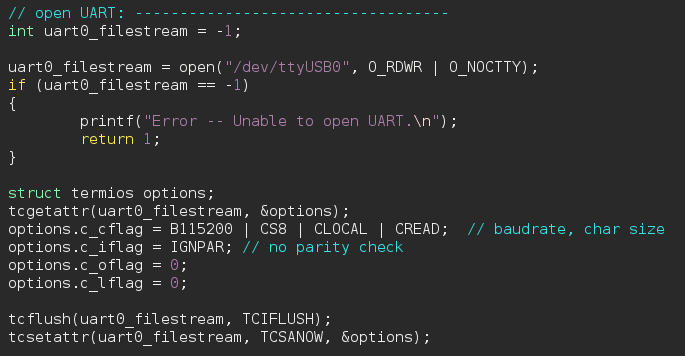
\includegraphics[scale=0.5]{images/uart.png}
    \caption{Konfiguracja portu szeregowego w języku C na systemie Linux.}
    \label{fig:uart}
  \end{center}
\end{figure}

Wysyłanie i odbieranie danych odbywa się za pomocą systemowych funkcji \texttt{read} i \texttt{write}, których używamy w dokładnie taki sam sposób, jak przy pisaniu do plików czy innych urządzeń wejścia/wyjścia. 
